\section[BOM和DOM的关系]{BOM和DOM的关系}
\begin{description}
  \item[BOM: ] Browser Object Model,没有统一标准
  \item[DOM: ] Document Object Model,有统一的标准
\end{description}

BOM和DOM的关系如图\ref{fig:bom_and_dom}和\ref{fig:bom_and_dom_2}所示。
\begin{figure}
  \centering
  % Requires \usepackage{graphicx}
  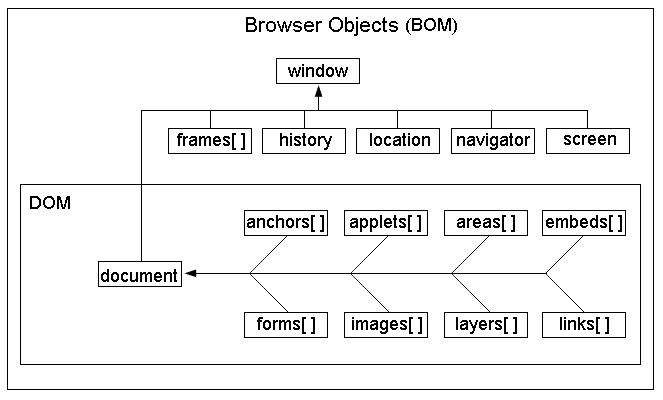
\includegraphics[width=.8\textwidth]{picturedir/js_bom_dom.jpg}\\
  \caption{BOM and DOM in JavaScript}\label{fig:bom_and_dom}
\end{figure}

\begin{figure}
  \centering
  % Requires \usepackage{graphicx}
  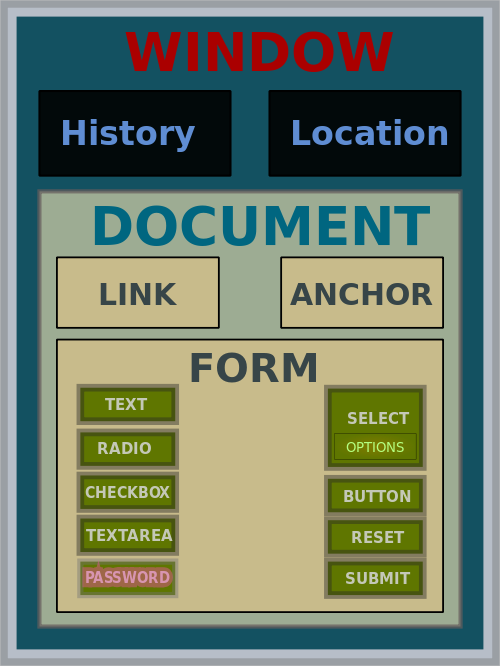
\includegraphics[width=.5\textwidth]{picturedir/js_bom_dom_2.png}\\
  \caption{BOM and DOM in JavaScript}\label{fig:bom_and_dom_2}
\end{figure}


\section[DOM是什么]{DOM是什么}
DOM(Document Object Model)是使用"JavaScript对象"来表示网页各个组成部分的方式。
网页被分解为一个个的node,最常用的是element nodes,attribute nodes和
text nodes三种,整个网页(the whole document)用document node来表示。

\section[获取页面元素]{获取页面元素}
获取页面元素有以下几种方式。
\subsection[Element ID]{Element ID}
\begin{javascriptcode}
  var widget = document.getElementById("widget");
  alert(widget);
\end{javascriptcode}

\subsection[Tag name]{Tag name}
\begin{javascriptcode}
  var pars = document.getElementsByTagName("p");
  for(var i = 0; i < pars.length; i++) {
    alert(pars[i]);
  }
\end{javascriptcode}

\subsection[Element name]{Element name}
\begin{javascriptcode}
  var widgetName = document.getElementsByName("widgetName")[0];
  alert(widgetName);
\end{javascriptcode}

\section[DOM node]{DOM node}
DOM将整个页面分解为node objects,所有的一切都是node object。
每个node都有三种属性:nodeType,nodeName,nodeValue。其中
nodeType用数字表示,如Node.ELEMENT\_NODE,nodeName用字符串表示,
如"H1"、"P"。

\subsection[Node之间的关系]{Node之间的关系}
所有的node都有下列属性:

\begin{itemize}
\item childNodes
\item firstChild
\item lastChild
\item nextSibling
\item previousSibling
\item parentNode
\end{itemize}

\subsection[获取node属性]{获取node属性}
第一种方式:通过node的".attributes"属性。

\begin{javascriptcode}
  <input type="text" name="widgetName" id="widget" />

  var output = '';
  var widget = document.getElementById("widget");
  var attrs = widget.attributes;
  for(var i = 0; i < attrs.length; i++) {
    output += attrs[i].name + '=' + attrs[i].value + '\n';
  }
  alert(output);
\end{javascriptcode}

第二种方法:getAttribute(name)

\begin{javascriptcode}
  var widget = document.getElementById('widget');
  alert(widget.getAttribute('type')); // display 'text'
  // or
  alert(widget.getAttributeNode('type')); // 打印node而不是其value
\end{javascriptcode}

当然,还可以预先判断某个属性是否存在:

\begin{javascriptcode}
  var isAttributeExists = elem.hasAttribute(attributeName);
\end{javascriptcode}

\subsection[修改node的属性]
改变属性值:

\begin{javascriptcode}
  <div>
    <img id="photo" src="cat.jpg" alt="My cat" />
  </div>

  var photo = document.getElementById('photo');
  var photoSrc = photo.getAttributeNode('src');
  var photoAlt = photo.getAttributeNode('alt');
  photoSrc.value = 'dog.jpg';
  photoAlt.value = 'My dog';
\end{javascriptcode}

增加属性:

\begin{javascriptcode}
  <div>
    <img id="photo" src="cat.jpg" alt="My cat" />
  </div>

  var photo = document.getElementById('photo');
  var width = document.createAttribute('width');
  width.value = 50;
  photo.setAttributeNode(width);
\end{javascriptcode}

快捷方式:

\begin{javascriptcode}
  // 如果name属性存在就修改其值,否则就增加name属性并设置其值为value
  elem.setAttribute(name, value);
\end{javascriptcode}

删除属性:

\begin{javascriptcode}
  //elem.removeAttribute(name);
  var photo = document.getElementById('photo');
  photo.setAttribute('width', 50);
  photo.removeAttribute('width');
\end{javascriptcode}


\subsection[修改node的值]{修改node的值}
修改node的值,只需修改node的nodeValue即可。

\begin{javascriptcode}
  <div id='welcome'> <p>Welcome to Widget.</p></div>
  var welcome = document.getElementById('welcome');
  welcome.firstChild.firstChild.nodeValue = 'Welcome U.';
\end{javascriptcode}

添加新的node:

\begin{javascriptcode}
  // 在尾部增加
  var welcome = document.getElementById('welcome');
  var horizRule = document.createElement('hr');
  welcome.appendChild(horizRule);
  // or
  // 在头部增加
  welcome.insertBefore(horizRule, welcome.firstChild);
\end{javascriptcode}

删除node:

\begin{javascriptcode}
  var welcome = document.getElementById('welcome');
  var horizRule = welcome.lastChild;
  welcome.removeChild(horizRule);
\end{javascriptcode}

替换node:

\begin{javascriptcode}
  var welcome = document.getElementById('welcome');
  var horizRule = welcome.lastChild;
  var newPar = document.createElement('p');
  newPar.appendChild(document.createTextNode('xxxxxx'));
  welcome.replaceChild(newPar, horizRule);
\end{javascriptcode}

移动node:

\begin{javascriptcode}
  <ul>
    <li id="widget1"><a href="superwidget.html">SuperWidget</a></li>
    <li id="widget2"><a href="megawidget.html">MegaWidget</a></li>
    <li id="widget3"><a href="wonderwidget.html">WonderWidget</a></li>
  </ul>
  // 只需将原来的node添加到需要的位置即可,旧的node自动删除,
  // 所以要想复制一个node就要使用createElement才行。
  var superWidget = document.getElementById("widget1");
  var ul = superWidget.parentNode;
  ul.appendChild(superWidget);
\end{javascriptcode}
